\section{Graded Assignment 3}\label{sec:graded_assignment_3}

% A full answer and result analysis is expected for task 3 and 4. For task 3 you should include a plot of the pose over time as well as the final estimated landmarks for your choice of parameters, in addition to NEES and NIS over time for the same set of parameters. In task 4 the same plots are expected, where the GPS can be used for ground truth. For both tasks it should be made clear why the parameters were chosen in terms of error metrics, consistency and overall result. Answers and analysis should connect theory and results to the real world, and show your understanding for the problem and solution. Try to connect the results on the simulated data to the results of the read data where and if it is possible. 

An extended Kalman filter was implemented for solving the SLAM problem in MATLAB. Specifically, the EKF-SLAM formulation in this report considers only the 2D case, with odometer measurements acting as control input. Furthermore, data association is done with the JCBB algorithm. For the relevant theory behind this EKF-SLAM formulation and JCBB, consult \cite[p. 185 - 196]{Edmund}.

\subsection{EKF-SLAM on simulated vehicle data set}

% Q, R, JCBB alphas
% NIS. Pose and lmks close to GT.

%The overall target was to minimize the difference between the estimated position and the ground truth, as well as decent NIS over time. Specifically we calculated the confidence interval over time with the size of the current innovation as the number of degrees of freedom. Initially, we set the noise covariance matrices higher than necessary, to get a rather conservative result, and decreased them as appropriatly. At the same time, we decreased the alphas used in the JCBB, as we could assume most of the measurements were from real landmarks. This resulted in a decently quick script, with the estimates being very close to the ground truth (with few / small offsets) and a decent NIS over time. 

The EKF-SLAM was first tuned using a simulated vehicle data set. The odometer measurement noise was tuned according to $Q = \text{diag}(\begin{array}{ccc}[(\sigma_u^2 & \sigma_v^2 & \sigma_\varphi^2 ]^{\top})\end{array}$, where $\sigma_u = \sigma_v = \SI{1e-1}{\meter\per\second}$ and $\sigma_\varphi = \SI{1e-2}{rad}$. The range-bearing measurement noise covariance was tuned according to $R = \text{diag}(\begin{array}{cc}[\sigma_r^2 & \sigma_\theta^2 ]^{\top})\end{array}$, where $\sigma_r = \SI{4e-2}{\meter}$ and $\sigma_\theta = \SI{2e-2}{rad}$. The JCBB algorithm was tuned by letting the individual compatability significance level be $\alpha_{ic} = \SI{1e-5}{}$ and the joint compatabiltiy significance level be $\alpha_{jc} = \SI{1e-10}{}$.

The system was tuned by trying to minimize the errors in pose and landmark estimates, while also looking at the calculated total NIS and NEES in pose. Note that in the NIS case the confidence interval was calculated at each time step, using the size of the current innovation as the number of degrees of freedom in the $\chi^2$ distribution. The estimated pose trajectory and landmark positions is presented in \cref{fig:ga_3_sim_trajectory}, and the consistency analysis plots are presented in \cref{fig:ga_3_sim_NIS}. We observe that 90\% of the NIS is inside the calculated the confidence interval, while 94.6\% of the NEES is inside the confidence intervals.

\begin{figure}[!htb]
    \centering
    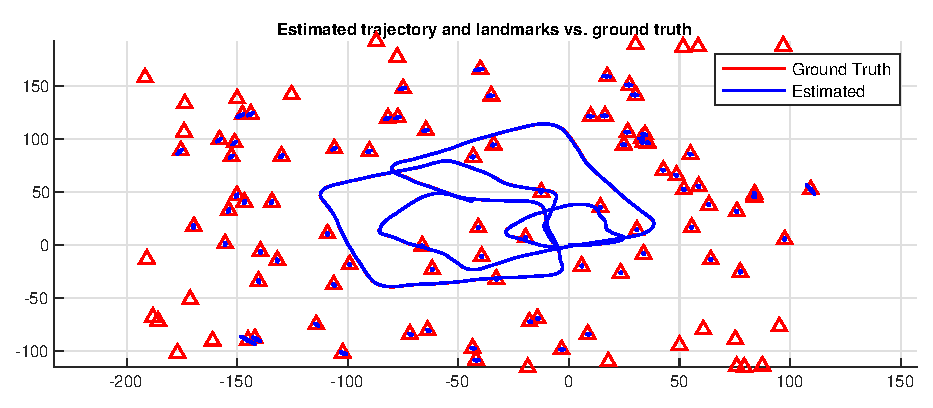
\includegraphics[width=0.7\linewidth]{figures/ga_3/sim_trajectory.eps}
    \caption{Estimated and ground truth pose trajectory and landmarks for simulated vehicle data}
    \label{fig:ga_3_sim_trajectory}
\end{figure}

\begin{figure}[!htb]
    \centering
    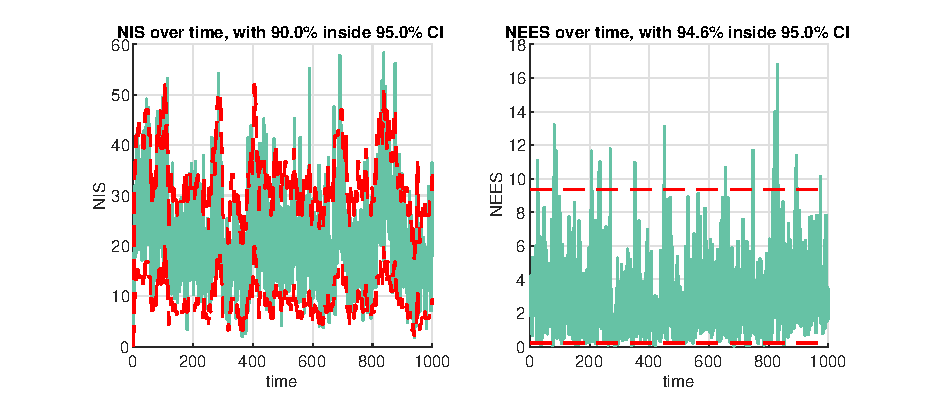
\includegraphics[width=0.9\linewidth]{figures/ga_3/sim_NIS.eps}
    \caption{Consistency for simulated vehicle data set with confidence intervals over time}
    \label{fig:ga_3_sim_NIS}
\end{figure}

Initially, the noise covariance matrices were set higher than necessary, to get a conservative result, and decreased until sufficient results were produced. At the same time, the compatibility alphas in the JCBB algorithm were reduced, as we could assume most of the measurements were from real landmarks.

% denseness, why?

%Discuss patterns in P - covariance. Discuss the two dots - why are these so high? They are not new states, but yet highly uncertain. It might just be the landmarks that are far away and that we have very few measurements off - might be the two landmarks with largest ellipses in trajectory plot? 
% Discuss using information matrix instead for speed? 

In \cref{fig:ga_3_sim_P} the covariance matrix and the inverse covariance matrix i.e. the information matrix at the last time step is presented. Talk about this...

\begin{figure}[!htb]
    \centering
    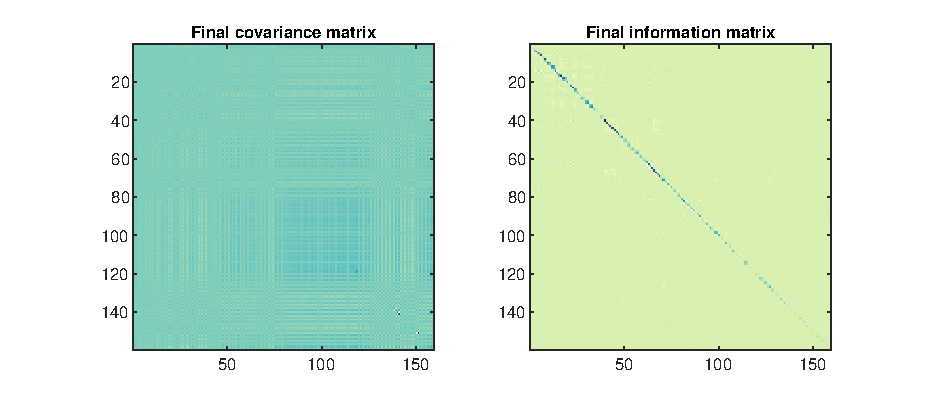
\includegraphics[width=0.8\linewidth]{figures/ga_3/sim_P.eps}
    \caption{Covariance matrix and information matrix for final timestep}
    \label{fig:ga_3_sim_P}
\end{figure}

% JCBB discussion

\subsection{EKF-SLAM on Victoria Park data set}

The EKF-SLAM code was then tested and tuned to the Victoria Park data set. The range-bearing measurement noise covariance was tuned with the same diagonal matrix, now with $\sigma_r = \SI{5e-2}{\meter}$ and $\sigma_\theta = \SI{5e-3}{rad}$. The odometer measurement noise covariance was now tuned to be
\begin{equation}
    Q = \begin{bmatrix}
        0.25 & 0 & 0 \\
        0 & 0.25 & 0.0225 \\
        0 & 0.0225 & 0.0025 \\
    \end{bmatrix}.
\end{equation}
The JCBB individual and joint compatability significance levels were now tuned to be $\alpha_{ic} = \SI{1e-3}{}$ and $\alpha_{jc} = \SI{1e-3}{}$.

The system was largely tuned by the same process as for the simulated data, but there are several differences worth mentioning. Firstly, the pose ground truth is naturally no longer available, only a GPS position signal. This was plotted in relation to the estimated pose trajectory and landmarks, as seen in \cref{fig:ga_3_real_trajectory}. But there is no easy way to properly compare the estimate to the GPS measurement, as the EKF-SLAM only produces a local estimate in relation to how it was initialized. In \cref{fig:ga_3_real_trajectory} the GPS measurements were therefore rotated until the two different frames looked somewhat aligned.

\begin{figure}[!htb]
    \centering
    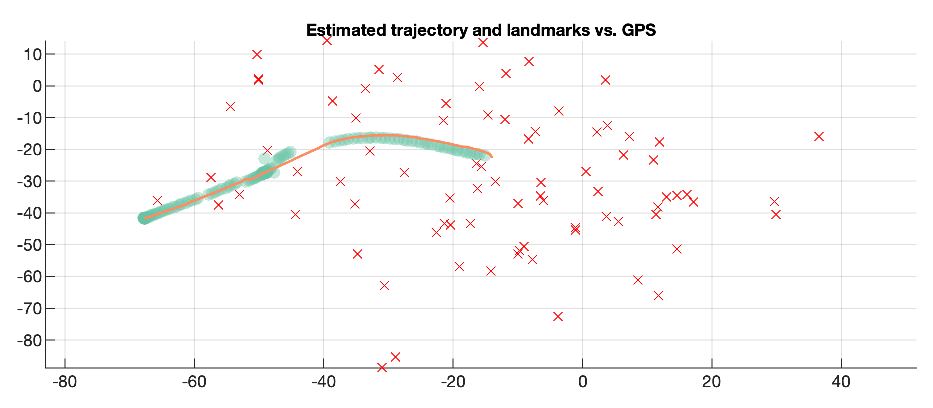
\includegraphics[width=0.7\linewidth]{figures/ga_3/real_trajectory.eps}
    \caption{Estimated pose trajectory, landmarks and GNSS measurements for Victoria Park data set}
    \label{fig:ga_3_real_trajectory}
\end{figure}

Since we no longer have the pose ground truth, the pose NEES is no longer available which also limits the available tools when tuning. But the NIS, again with a variable degree of freedom confidence interval, was actively used and is presented for the final tuning parameters in \cref{fig:ga_3_real_NIS}. It was calculated that 67\% of the NIS was inside the confidence intervals.  

\begin{figure}[!htb]
    \centering
    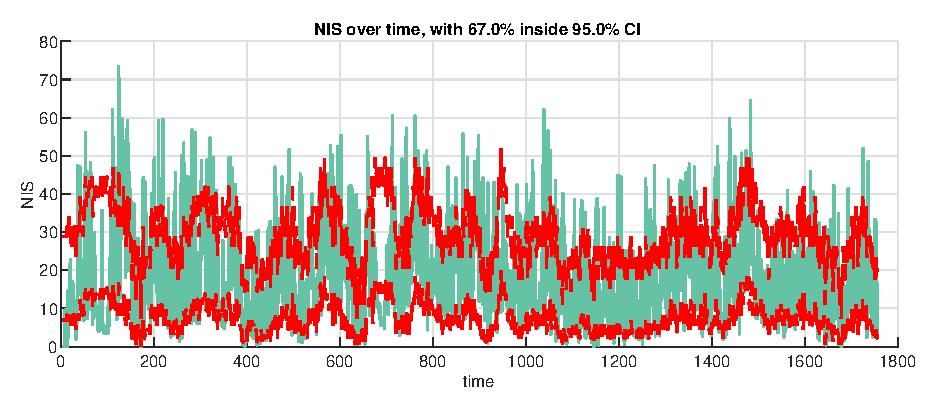
\includegraphics[width=0.8\linewidth]{figures/ga_3/real_NIS.eps}
    \caption{NIS for Victoria Park data set with confidence intervals over time}
    \label{fig:ga_3_real_NIS}
\end{figure}

One should also note the much higher compatibility alphas compared to the simulated data set. It was quickly observed while testing the system that the spread in range-bearing measurements of the landmarks was larger compared to the simulated case. It was concluded that the JCBB gating that was previously used was too low for this data set, and therefore increased.

% discuss EKF-SLAM assumptions.
% Discuss performance of EKF-SLAM. Why it sucks ass. Improvements? 